\documentclass[11pt]{article}

\usepackage[margin=1in]{geometry}
\usepackage{amsmath, amssymb}
\usepackage{booktabs}
\usepackage{graphicx}
\usepackage{natbib}
\usepackage{setspace}
\usepackage{hyperref}
\usepackage{caption}

\hypersetup{colorlinks=true, citecolor=blue, linkcolor=blue, urlcolor=blue}
\setlength{\parskip}{0.5em}
\doublespacing

\title{Drive-Level Momentum in the NFL: \\
       \large Most of It Is Short Fields, and the Residual Cuts the Other Way}

\author{Jonathan Walberg\\University of Virginia}
\date{\today}

\begin{document}
\maketitle

\begin{abstract}
\noindent Coaches, broadcasters, and fans treat NFL momentum as a within-team
phenomenon, but the data, properly disaggregated, place the action between
teams. Using \texttt{nflfastR} play-by-play covering 4{,}078 games and
85{,}955 drives from 2010--2024, I decompose drive-to-drive momentum into
three channels: own-team defensive-stop spillover (H1), own-team offensive
carryover (H2), and opponent suppression (H3). The unconditional H1 gap is
large (52.2\% vs.\ 35.6\%, a 16.6-percentage-point difference). Once starting
field position and game-state controls are added, along with game and
possessing-team fixed effects, H1 collapses to 2.0 points and H2 turns
negative ($-4.2$ points), reversing the broadcast prediction. The
opponent-suppression channel survives all controls and is large in magnitude:
scoring probability is 32.7 percentage points lower following an opponent
score (a logit comparison without game fixed effects returns a smaller but
qualitatively identical effect). A battery of eight robustness checks
--- including flexible field-position controls, a
post-touchdown-versus-post-field-goal placebo, a logit comparison,
within-team-quarter permutation inference, and a rule-era split ---
indicates that the cross-team channel is not a linear-control artifact.
The within-team channels collapse under the same controls. To my knowledge,
this is the first peer-reviewed drive-level NFL test of momentum and the
first to separate within-team from cross-team channels.

\medskip
\noindent\textbf{Keywords:} momentum; hot hand; play-by-play; fixed effects;
nflfastR; cross-team spillover
\end{abstract}

\section{Introduction}

The single most invoked, least defined construct in football broadcasting is
momentum. The empirical case for any of it is thinner than the usage suggests,
but the way the construct is described in coaching, broadcasting, and fan
discussion mixes three propositions that have different observable
implications and that the data treat very differently. Pulling them apart
makes a sharp contrast visible: drive-to-drive momentum, properly defined,
splits into a small-or-wrong-signed within-team component and a large cross-team
component, and what broadcasts call momentum is overwhelmingly a description
of the latter.

The hot-hand literature originated in basketball with
\citet{gilovich1985hot}'s finding that perceived shooting streaks were a
perceptual artifact: shooters' makes and misses behave like independent
Bernoulli trials. The claim held as a benchmark for three decades until
\citet{miller2018surprised} identified a selection bias in the original test.
With the bias correction, modest positive streak effects appear in the
original Cornell shooting data. In team sports, the question divides further:
do team-level outcomes (a win, a score, a turnover) influence the team's next
outcome of the same kind, or are sequences of game events independent given
the underlying quality of the teams playing?

For the NFL, to my knowledge in the peer-reviewed literature the only direct test in the \emph{Journal of
Quantitative Analysis in Sports} is \citet{fry2012searching}, who examine NFL
momentum at the level of full games and find no evidence that recent wins
predict future wins above what team strength can explain.
\citet{arkes2011finally} make a parallel test for the NBA and report that,
after correcting for opponent strength and home-court advantage, NBA teams
that win their previous game are modestly more likely to win the next.
\citet{steeger2021winning} apply an entropy test to NHL season-level streaks
and reject momentum at that scale. \citet{lopez2018often} use a unified
generalized linear mixed-model framework to compare randomness in outcomes
across the four major North American sports and find that NFL outcomes are
the most randomness-driven among them, consistent with weak game-level
momentum signals.

Game-level tests answer a different question than the one coaches actually
care about. A coach calling a timeout in the third quarter is not making an
inference about whether wins predict wins across a 17-game season; the
inference is that something on the field has shifted, in this game, in a way
that will carry into the next drive. The natural unit at which to test that
inference is the drive, and the natural data source is the modern play-by-play
record curated through \citet{yurko2018nflwar} and now distributed via the
\texttt{nflfastR} R package \citep{nflfastr2024}.

This paper uses 4{,}078 NFL games and 85{,}955 drives over the 2010--2024
seasons to decompose drive-to-drive momentum into three channels that mirror
the way the construct is invoked in real time:

\begin{enumerate}
    \item[\textbf{H1.}] \emph{Defensive-stop spillover} --- A team's offensive
    drive is more likely to end in a score when the team's defense forced a
    drive of three or fewer plays ending in a punt, an interception, a fumble
    lost, a turnover on downs, or a safety on the immediately preceding drive.
    \item[\textbf{H2.}] \emph{Offensive carryover} --- A team's offensive drive
    is more likely to end in a score when the team's previous offensive drive
    ended in a score.
    \item[\textbf{H3.}] \emph{Opponent suppression} --- A team's offensive
    drive is \emph{less} likely to end in a score when the opponent's previous
    drive ended in a score.
\end{enumerate}

The substantive finding is that the unconditional version of H1 is large in
the way coaches and broadcasters describe it --- scoring probability is
52.2\% after a defensive stop versus 35.6\% otherwise --- but most of that gap
is the mechanical short-field effect of turnovers and quick punts combined
with the behavior of the comparison group, which mixes opponent scores into
the ``not-a-stop'' bucket. Once starting field position and standard game-state
controls are added, along with game and possessing-team fixed effects, the
H1 effect collapses to 2.0 percentage points. H2 reverses sign: a prior own
scoring drive is associated with a 4.2-percentage-point \emph{decline} in the
next own drive's scoring probability, potentially explained by mechanisms such
as regression to the mean and in-game defensive adjustment, neither of which
the present design can isolate. H3 survives every control and is the largest
residual: conditional on starting field position, scoring probability
following a drive on which the opponent scored is 32.7 percentage points lower
than following a non-scoring opponent drive. This is the only channel where
the data behave like the construct broadcasters have in mind --- and it is
not the team that just scored that carries it; it is the team that was just
scored on that loses ground.

The paper proceeds as follows. Section \ref{sec:lit} situates the analysis
relative to the existing JQAS work on NFL momentum and the broader hot-hand
literature. Section \ref{sec:theory} develops the three channels and makes
the identification problem explicit. Section \ref{sec:data} describes the
data and the construction of drive-level outcomes from play-by-play.
Section \ref{sec:strategy} states the estimation strategy. Section
\ref{sec:results} presents the main results and a robustness gauntlet
designed specifically to discriminate cross-team psychological residue from
linear-control artifact. Section \ref{sec:discuss} discusses what the results
imply for in-game decision making and for the academic literature on
team-sport momentum. Section \ref{sec:concl} concludes.

\section{Related Literature}\label{sec:lit}

The hot-hand literature begins with \citet{gilovich1985hot}.
\citet{miller2018surprised}'s correction to the original test is now a
benchmark; \citet{bareli2006twelve} provide a comprehensive review of the
intervening twelve years of hot-hand research and the methodological turn it
has taken, including the sport-psychology literature that grounds coaches'
priors about momentum. The sport-psychology tradition treats momentum as a
real psychological state that influences subsequent execution, while the
statistical hot-hand tradition treats apparent streaks as samples from an
independent process given underlying team quality. This paper sits closer to
the statistical tradition methodologically but uses a unit of analysis (the
drive) and a construct (cross-team spillover) that the sport-psychology
literature has long argued is where the real action is.

For team sports, the unit of analysis matters. \citet{stern1994probabilities}
modeled in-game score progression as a Brownian motion, implying conditional
score paths are largely random walks given team strengths.
\citet{berger2011hot} look across the NBA, NCAA football, and lab experiments
and find that being slightly behind at halftime increases the probability of
winning, which they interpret as a motivational-effort response rather than
a chance pattern. \citet{csapo2014hand} use novel defense metrics to show
that NBA defenses adjust to perceived hot streaks, which complicates the
interpretation of within-team streaks even when they appear in the data.
\citet{gauriot2019does} use a quasi-experimental tennis design and find that
strategic momentum operates between players in dynamic contests, the closest
prior result to this paper's H3 finding in spirit.

Within JQAS specifically, three momentum studies anchor the literature.
\citet{arkes2011finally} use NBA game-level data and report that prior-game
outcomes predict next-game outcomes after controlling for team strength and
home-court advantage, contrary to the standard hot-hand-fallacy claim.
\citet{steeger2021winning} apply an entropy measure to NHL season-level win
sequences and conclude that the streak structure is consistent with random
events given team strength. \citet{fry2012searching} is the only direct test
on NFL data and finds no evidence for game-to-game momentum. None of these
works addresses momentum at the drive level.

The methodological tools for a drive-level test now exist.
\citet{yurko2018nflwar} introduced the \texttt{nflscrapR} pipeline that
produces clean play-by-play records with fixed-drive identifiers, EPA values,
and win-probability estimates; \citet{nflfastr2024}'s \texttt{nflfastR}
extended the data back to 1999 and made it the field standard for NFL
play-by-play research. Drive-level work in JQAS includes
\citet{goldner2012markov}'s Markov model of drive progression,
\citet{cafarelli2012third}'s analysis of third-down conversion,
\citet{lock2014random}'s random-forest win-probability model,
\citet{yam2019what}'s causal estimate of the cost of conservative fourth-down
behavior, and \citet{brill2024expected}'s recent re-examination of
expected-points estimation. Closely related, \citet{kovash2009professional}
reanalyze NFL play-calling and find evidence consistent with non-equilibrium
behavior, suggesting that play-level decisions are not always optimally
randomized. None of these papers tests momentum.

\section{Theory and Hypotheses}\label{sec:theory}

The way ``momentum'' is described on broadcasts and in postgame press
conferences turns out to mix three distinct propositions. Pulling them apart
matters because they have different observable implications and different
identification problems.

\paragraph{Channel 1 --- Defensive-stop spillover.} The claim is that when
a defense forces a drive ending in a punt of three or fewer plays, an
interception, a fumble lost, a turnover on downs, or a safety, the offense
it sends back onto the field plays better than it would otherwise. This is
the version of momentum that motivates calls like ``the defense just gave the
offense a spark.'' The observational pattern is unambiguous in the raw data
--- teams score more often after defensive stops --- but the same data are
also unambiguous about why: stops, especially turnovers, give the offense a
shorter field. Distinguishing momentum from mechanics requires conditioning
on starting field position and on the comparison group's composition.

\paragraph{Channel 2 --- Offensive carryover.} The claim is that scoring
breeds scoring on subsequent possessions by the same offense. Two competing
hypotheses are observationally consistent with the absence of carryover:
regression to the mean (a scoring drive draws from the upper tail of a team's
drive-quality distribution and the next drive will tend to draw from closer
to the mean) and in-game defensive adjustment (an opponent now playing from
behind may shift to more aggressive schemes that the just-scoring offense has
not yet adapted to). Both predict a non-positive coefficient on prior own
offensive scoring; the present design cannot adjudicate between them.

\paragraph{Channel 3 --- Opponent suppression.} The claim is that a team that
has just been scored on is briefly demoralized, less crisp on its next
possession, and more prone to mistakes. The competing hypothesis is again
mechanical: after a touchdown or field goal, the scored-on team starts the
next drive at the kickoff-touchback yardline, which is a different starting
field position than after the opponent punted or turned the ball over.
Conditional on starting field position and game state, however, any residual
gap is the psychological component the broadcast usually has in mind. An
important caveat is that the linear field-position control may not fully
absorb the distributional asymmetry between the post-kickoff regime
(concentrated near the touchback yardline) and the post-punt or
post-turnover regime (spread across the field); Section
\ref{sec:results} reports a battery of robustness checks designed
specifically to address this concern.

The three channels share an identification problem: the sequence of drives
within a game is not an independent draw. Field position, score differential,
time remaining, and the opponent's recent behavior all evolve jointly with
the channels of interest. The estimation strategy below addresses this by
controlling for game state, by absorbing game-level fixed effects, and by
including possessing-team fixed effects so that comparisons are within
team-game cells rather than across them.

\section{Data}\label{sec:data}

\subsection{Source}

Play-by-play data come from \texttt{nflfastR} \citep{nflfastr2024}, which
distributes the fixed-drive--enriched version of the original
\texttt{nflscrapR} pipeline \citep{yurko2018nflwar}. The sample covers
regular-season and postseason games from 2010 through 2024, yielding 721{,}566
plays across 4{,}078 games. Plays are aggregated to the drive level using the
\texttt{fixed\_drive} identifier, which corrects irregularities in the raw
NFL drive numbering. After dropping plays with missing drive identifiers,
end-of-half kneel-down drives, end-of-game drives, and drives missing the
core analysis fields (offensive outcome, starting field position, score
differential), the analysis dataset contains 85{,}955 offensive drives.

\subsection{Outcome variables}

The primary outcome is a binary indicator for whether a drive ended in a
score (touchdown or field goal). Across the sample, 38.1\% of drives end in
a score. As a robustness check, I also use the sum of expected-points-added
(EPA) on the drive as a continuous outcome.

\subsection{Momentum indicators}

The three channels require three distinct lagged indicators, each defined
relative to the team currently in possession.

\begin{itemize}
    \item \textbf{Prior own-defensive success.} Equal to one if the
    immediately preceding drive (the opponent's offensive possession) ended in
    a punt with three or fewer plays, an interception, a fumble lost, a
    turnover on downs, or a safety.
    \item \textbf{Prior own-offensive success.} Equal to one if the same
    team's most recent prior offensive drive ended in a touchdown or field
    goal. The walk-back through prior drives skips intervening opponent
    possessions.
    \item \textbf{Prior opponent-offensive success.} Equal to one if the
    opponent's most recent prior offensive drive ended in a touchdown or field
    goal.
\end{itemize}

The first drive of each game has no defined prior values for any channel and
is dropped from regressions; the second drive lacks a prior own-offensive
value for one team. After requiring all three indicators to be defined, the
estimation sample contains 73{,}842 drives.

\subsection{Controls}

Drive starting field position is recorded as \texttt{yardline\_100} (yards
from the opponent's end zone, 100 = own goal line). Game state controls
include the score differential at drive start, quarter, half-seconds
remaining, and a home-team indicator. The main specification absorbs game
and possessing-team fixed effects.

\section{Estimation Strategy}\label{sec:strategy}

The main specification is a linear probability model for drive $d$ played
by possessing team $k$ in game $g$:

\begin{equation}\label{eq:main}
    \text{Score}_{dkg} = \alpha_g + \gamma_k + \beta_1 D_{dkg}^{\text{def}} +
    \beta_2 D_{dkg}^{\text{own-off}} + \beta_3 D_{dkg}^{\text{opp-off}} +
    X_{dkg}'\delta + \varepsilon_{dkg},
\end{equation}

where $\text{Score}_{dkg}$ is one if drive $d$ by team $k$ in game $g$ ended
in a score, $\alpha_g$ is a game fixed effect, $\gamma_k$ is a possessing-team
fixed effect, $D^{\text{def}}, D^{\text{own-off}}, D^{\text{opp-off}}$ are the
three momentum indicators (corresponding to H1, H2, and H3, respectively),
and $X_{dkg}$ is a column vector stacking starting field position, score
differential, quarter, half-seconds remaining, and the home indicator, with
$\delta$ the conformable coefficient vector. Identification of $\beta_1,
\beta_2, \beta_3$ relies on within-game, within-team variation in the three
lagged indicators conditional on $X$. Game and possessing-team fixed effects
are jointly identified because each game contains two distinct possessing
teams, so $\alpha_g$ and $\gamma_k$ are not collinear within a game.

Standard errors are two-way clustered by game and possessing team
\citep{cameron2011robust} to handle within-game serial correlation in drive
outcomes and within-team correlation across games. The linear probability
model is preferred to logit because the fixed-effect structure is
high-dimensional (one fixed effect per game, plus 32 team fixed effects), and
the marginal-effect interpretation maps directly onto the percentage-point
quantities coaches care about. Section \ref{sec:robust} reports a logit
comparison and the share of LPM predicted probabilities that fall outside
$[0,1]$.

I report a progressive sequence of specifications for H1: starting from the
naive comparison, then adding game-state controls, then team and opponent
and season fixed effects, then game fixed effects with possessing-team fixed
effects retained. The progression shows how much of the apparent H1 effect
is mechanical versus residual; the prior JQAS work performs this
decomposition only at the game level.

\section{Results}\label{sec:results}

\subsection{The unconditional gap is large}

Table \ref{tab:descrip} reports the raw conditional means. The probability
of a scoring drive is 52.2\% when the team's defense just produced a stop
and 35.6\% otherwise --- a 16.6-percentage-point gap. The probability of a
scoring drive is 35.2\% when the opponent's prior drive ended in a score and
40.0\% otherwise --- a 4.8-percentage-point gap of the predicted sign.
Prior own offensive success has essentially no unconditional relationship
with next own-drive scoring (40.3\% vs.\ 37.0\%, gap of 3.3 percentage points).

\begin{table}[htbp]
\centering
\caption{Unconditional drive-level scoring probabilities by prior context.}
\label{tab:descrip}
\begin{tabular}{lcc}
\toprule
Condition & P(score) & N drives \\
\midrule
After own defensive stop & 0.522 & 11,782 \\
After opponent score or longer punt & 0.356 & 66,137 \\
\midrule
After own offensive score (prior own drive) & 0.403 & 28,505 \\
After own offensive non-score & 0.370 & 49,384 \\
\midrule
After opponent score (prior opp drive) & 0.352 & 31,129 \\
After opponent non-score & 0.400 & 50,684 \\
\bottomrule
\end{tabular}
\\[0.5em]
\begin{minipage}{0.95\textwidth}
\footnotesize
\textit{Notes.} Each panel uses the largest sample for which the relevant prior-drive indicator is defined; sample size therefore differs across panels (the unified estimation sample requiring all three indicators is N = 73{,}842 drives). Sample: NFL regular season + postseason 2010--2024 from nflfastR. 
\end{minipage}
\end{table}


\subsection{Decomposing H1: most of the gap is the comparison group, not the field}

Figure \ref{fig:fp} plots the scoring probability by drive starting field
position decile, separately for drives following defensive stops and drives
following normal opponent possessions. At the goal-line decile (drives
starting inside the opponent 10), the two curves converge near 90\%. At the
own-end-zone decile (drives starting inside the team's own 10), the curves
converge near 24\%. The visible gap between the curves is concentrated at
mid-field starting positions, where stop-following drives are
disproportionately distributed.

\begin{figure}[htbp]
\centering
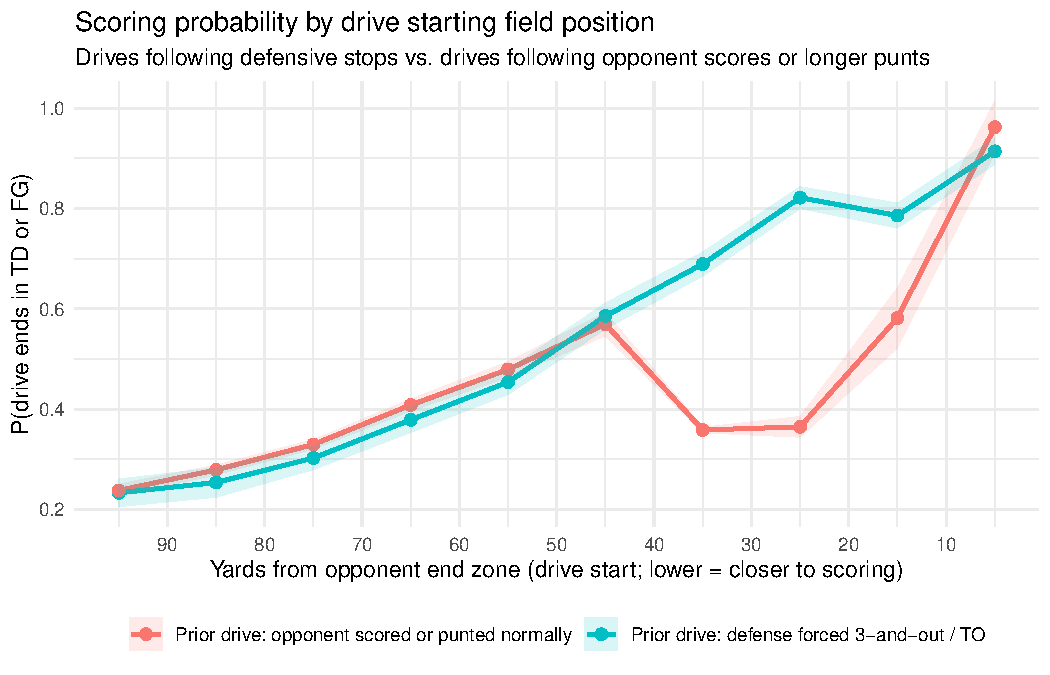
\includegraphics[width=0.85\textwidth]{figures/fig1_field_position.pdf}
\caption{Scoring probability by drive starting field position, conditional on
whether the prior drive was a defensive stop. Sample: drives in the
73{,}842-drive estimation sample for which a prior own-defensive indicator is
defined; data from \texttt{nflfastR} \citep{nflfastr2024}, NFL 2010--2024.
The $x$-axis is yards from the opponent end zone (lower = closer to scoring),
binned into deciles; the $y$-axis is the empirical probability of the drive
ending in a touchdown or field goal. Solid line: drives following a defensive
stop. Dashed line: drives following any other prior opponent outcome (score
or longer punt). Shaded bands show 95\% pointwise binomial confidence
intervals. The unconditional 16.6-percentage-point gap is concentrated in
the middle deciles, where stop-following drives are over-represented. At the
extremes the curves converge: a drive that starts inside the opponent 10
scores roughly 90\% of the time regardless of how it got there, and a drive
that starts inside the own 10 scores roughly 24\% regardless.}
\label{fig:fp}
\end{figure}

Table \ref{tab:h1prog} formalizes the same decomposition through a sequence
of regressions. Column 1 is the naive comparison: the H1 coefficient is
16.3 percentage points (s.e.\ 0.5). Adding game-state controls in column 2
--- field position, score differential, quarter, time, home --- brings the
coefficient down to 14.7 points. Adding team, opponent, and season fixed
effects in column 3 leaves it at 14.7 points. Switching to game fixed effects
while retaining possessing-team fixed effects (and dropping opponent and
season fixed effects) in column 4 yields 17.4 points: within games, drives
following defensive stops score more often than other drives in the same
game, mostly because they follow events that systematically differ from the
events preceding the comparison drives. Possessing-team fixed effects are
identified within game because each game contains two distinct possessing
teams.


\begin{table}[htbp]
   \caption{\label{tab:h1prog} Defensive Stop Spillover (H1): Progressive Controls. \textit{Notes.} OLS linear probability models. Dependent variable is an indicator for whether the drive ends in a touchdown or field goal. Sample: NFL regular season + postseason 2010--2024 (nflfastR). Game-state controls (field position, score differential, quarter, half-seconds remaining, home indicator) included in columns 2--4 with coefficients suppressed for readability. Standard errors in parentheses, two-way clustered by game and possessing team \citep{cameron2011robust}. $^{*}p<0.10$, $^{**}p<0.05$, $^{***}p<0.01$.}
   \centering
   \begin{tabular}{lcccc}
      \tabularnewline \midrule \midrule
      Dependent Variable: & \multicolumn{4}{c}{Drive ends in score (0/1)}\\
      Model:                                  & (1)            & (2)                           & (3)                           & (4)\\  
      \midrule
      \emph{Variables}\\
      Constant                                & 0.3562$^{***}$ & 0.5348$^{***}$                &                               &   \\   
                                              & (0.0062)       & (0.0095)                      &                               &   \\   
      Prior own defensive stop                & 0.1626$^{***}$ & 0.1466$^{***}$                & 0.1470$^{***}$                & 0.1735$^{***}$\\   
                                              & (0.0055)       & (0.0052)                      & (0.0052)                      & (0.0055)\\   
      Field position (yards to opp. end zone) &                & -0.0029$^{***}$               & -0.0029$^{***}$               & -0.0021$^{***}$\\   
                                              &                & ($7.74\times 10^{-5}$)        & ($7.81\times 10^{-5}$)        & ($7.52\times 10^{-5}$)\\    
      Score differential                      &                & 0.0017$^{***}$                & 0.0012$^{***}$                & 0.0012$^{***}$\\   
                                              &                & (0.0002)                      & (0.0001)                      & (0.0002)\\   
      Quarter                                 &                & -0.0134$^{***}$               & -0.0132$^{***}$               & -0.0139$^{***}$\\   
                                              &                & (0.0015)                      & (0.0014)                      & (0.0016)\\   
      Half seconds remaining                  &                & $1.38\times 10^{-5}$$^{***}$  & $1.44\times 10^{-5}$$^{***}$  & $1.56\times 10^{-5}$$^{***}$\\    
                                              &                & ($3.17\times 10^{-6}$)        & ($3.16\times 10^{-6}$)        & ($3.39\times 10^{-6}$)\\    
      Home offense                            &                & 0.0245$^{***}$                & 0.0253$^{***}$                &   \\   
                                              &                & (0.0036)                      & (0.0036)                      &   \\   
      \midrule
      \emph{Fixed-effects}\\
      Possessing team                         &                &                               & Yes                           & Yes\\  
      Opponent                                &                &                               & Yes                           & \\  
      Season                                  &                &                               & Yes                           & \\  
      Game                                    &                &                               &                               & Yes\\  
      \midrule
      \emph{Fit statistics}\\
      Observations                            & 73,842         & 73,842                        & 73,842                        & 73,842\\  
      R$^2$                                   & 0.01455        & 0.03554                       & 0.04303                       & 0.09511\\  
      Within R$^2$                            &                &                               & 0.03434                       & 0.02938\\  
      \midrule \midrule
      \multicolumn{5}{l}{\emph{Clustered (Game \& Possessing team) standard-errors in parentheses}}\\
      \multicolumn{5}{l}{\emph{Signif. Codes: ***: 0.01, **: 0.05, *: 0.1}}\\
   \end{tabular}
\end{table}




The 14.7-to-17.4-percentage-point range across columns 2--4 looks like
substantial within-team momentum until the other two channels are added.
Adding the other channels reveals that the H1 coefficient absorbs the
contrast between drives following defensive stops and drives following
opponent scores; once the latter is moved into a separate H3 channel, the
residual H1 channel is small. Of the 16.6-percentage-point unconditional
gap, only about 1.6 percentage points is absorbed by the linear field-position
control alone (the difference between columns 1 and 2 of Table
\ref{tab:h1prog}). The bulk of the collapse from 16.3 to 2.0 percentage
points comes from re-classifying the comparison group: the ``not a stop''
bucket in the H1-only model mixes opponent scores into the comparison, and
moving opponent scores into a dedicated H3 channel reveals the H1 residual
to be small.

\subsection{Joint estimation: the headline}\label{sec:joint}

Table \ref{tab:allchan} reports the joint estimation. Column 1 is the
preferred specification, equation \eqref{eq:main}, with all three momentum
indicators, full game-state controls, game fixed effects, and possessing-team
fixed effects.


\begin{table}[htbp]
   \caption{\label{tab:allchan} Three Momentum Channels: Joint Estimation and Robustness. \textit{Notes.} Column 1 is the preferred specification: linear probability model for whether the drive ends in a score, with all three momentum indicators jointly. Column 2 drops drives in garbage time (absolute score differential $\geq 21$ in the fourth quarter). Column 3 replaces the binary outcome with the sum of expected-points-added (EPA) on the drive. All columns include game-state controls (field position, score differential, quarter, half-seconds remaining) and game and possessing-team fixed effects. Standard errors in parentheses, two-way clustered by game and possessing team \citep{cameron2011robust}. $^{*}p<0.10$, $^{**}p<0.05$, $^{***}p<0.01$.}
   \centering
   \begin{tabular}{lccc}
      \tabularnewline \midrule \midrule
      Dependent Variables: & \multicolumn{2}{c}{Drive ends in score (0/1)} & Drive EPA\\
      Model:                                  & (1)                            & (2)                            & (3)\\  
      \midrule
      \emph{Variables}\\
      Prior own defensive stop                & 0.0204$^{***}$                 & 0.0239$^{***}$                 & -0.1650$^{***}$\\   
                                              & (0.0063)                       & (0.0067)                       & (0.0437)\\   
      Prior own offensive score               & -0.0423$^{***}$                & -0.0461$^{***}$                & -0.2417$^{***}$\\   
                                              & (0.0039)                       & (0.0037)                       & (0.0313)\\   
      Prior opponent offensive score          & -0.3271$^{***}$                & -0.3248$^{***}$                & -0.5034$^{***}$\\   
                                              & (0.0063)                       & (0.0067)                       & (0.0530)\\   
      Field position (yards to opp. end zone) & -0.0067$^{***}$                & -0.0067$^{***}$                & -0.0032$^{***}$\\   
                                              & (0.0001)                       & (0.0001)                       & (0.0008)\\   
      Score differential                      & 0.0003$^{*}$                   & 0.0007$^{***}$                 & 0.0012\\   
                                              & (0.0002)                       & (0.0002)                       & (0.0014)\\   
      Quarter                                 & -0.0163$^{***}$                & -0.0128$^{***}$                & -0.0976$^{***}$\\   
                                              & (0.0018)                       & (0.0020)                       & (0.0126)\\   
      Half seconds remaining                  & $-1.37\times 10^{-5}$$^{***}$  & $-1.85\times 10^{-5}$$^{***}$  & $-5.72\times 10^{-5}$$^{*}$\\    
                                              & ($3.75\times 10^{-6}$)         & ($3.7\times 10^{-6}$)          & ($2.87\times 10^{-5}$)\\    
      \midrule
      \emph{Fixed-effects}\\
      Game                                    & Yes                            & Yes                            & Yes\\  
      Possessing team                         & Yes                            & Yes                            & Yes\\  
      \midrule
      \emph{Fit statistics}\\
      Observations                            & 73,842                         & 71,090                         & 73,842\\  
      R$^2$                                   & 0.13389                        & 0.13544                        & 0.07815\\  
      Within R$^2$                            & 0.07098                        & 0.07086                        & 0.00417\\  
      \midrule \midrule
      \multicolumn{4}{l}{\emph{Clustered (Game \& Possessing team) standard-errors in parentheses}}\\
      \multicolumn{4}{l}{\emph{Signif. Codes: ***: 0.01, **: 0.05, *: 0.1}}\\
   \end{tabular}
\end{table}




The joint H1 coefficient is 2.0 percentage points (s.e.\ 0.6, $p<0.01$). It
is statistically significant in this large sample but substantively small:
about one-eighth of the raw conditional difference, and far below the level
that would justify the broadcaster description of a defensive stop
``shifting momentum.''

The joint H2 coefficient is $-4.2$ percentage points (s.e.\ 0.4, $p<0.001$).
The negative sign rejects the simplest version of the offensive-carryover
claim. A team's prior own-offensive scoring drive is associated with a
4.2-percentage-point lower probability that its next own-offensive drive
will score, conditional on game and field-position controls. Two
non-exclusive mechanisms are consistent with the negative sign --- regression
to the mean and in-game defensive adjustment --- but the present design
cannot adjudicate between them or rule out alternatives.

The joint H3 coefficient is $-32.7$ percentage points (s.e.\ 0.6, $p<0.001$).
This is the largest of the three effects by a wide margin and the only one
in the direction that the broadcast usage of momentum would predict. After
conditioning on starting field position, score differential, time remaining,
and team and game fixed effects, the team that has just been scored on is
much less likely to score on its next drive than the team that just survived
a punt or a defensive stop. Two caveats are important. First, the linear
field-position control may not fully absorb the distributional asymmetry
between drives starting after a kickoff (concentrated near the touchback
yardline) and drives starting after a punt or turnover (spread across the
field); the robustness analyses in Section \ref{sec:robust} address this
concern directly. Second, the design does not rule out unobserved
within-game shocks (e.g., an injury that occurs during or shortly before the
opponent's scoring drive and degrades the offense's next possession) that
would correlate being-scored-on with subsequent suppression; this caveat is
discussed further in Section \ref{sec:limits}.\footnote{An interactive
companion supplement showing the three-channel decomposition is provided
with the replication package at \texttt{figures/interactive/nfl\_three\_channels.html}.}

\subsection{Robustness}\label{sec:robust}

I report eight robustness checks designed specifically to discriminate
linear-control artifact from the cross-team residual the H3 coefficient is
meant to identify. The full set of estimates is documented in
\texttt{data/robustness.rds}; the headline numbers are summarized below.

\paragraph{R1. Flexible field-position and score-differential controls.}
Replacing the linear $\texttt{yardline\_100}$ control with field-position
decile fixed effects and the linear $\texttt{score\_differential}$ control
with 10-bin score-margin dummies leaves H3 substantially unchanged at
$\hat\beta_3^{\text{flex}} = -28.4$ percentage points (s.e.\ 0.9). The
flexible specification absorbs roughly 4 of the original 32.7 percentage
points, indicating that the bulk of the H3 effect is not a
linear-functional-form artifact in the field-position control.

\paragraph{R2. Placebo: post-touchdown vs.\ post-field-goal.} Restricting
the sample to drives following an opponent score (touchdown or field goal),
both of which produce a kickoff regime, and regressing scoring probability
on a post-touchdown indicator (with the post-field-goal cell as the omitted
category) yields a coefficient of $-0.8$ percentage points (s.e.\ 0.7;
$N = 27{,}615$). The null coefficient indicates that, conditional on game
and team controls, post-touchdown and post-field-goal drives score at
similar rates within the post-score regime; H3 does not appear to require
a touchdown-specific demoralization story.

\paragraph{R3. Logit comparison and LPM out-of-bounds check.} The share of
LPM predicted probabilities outside $[0,1]$ is small (0.45\% below 0;
0.20\% above 1; 0.65\% total). Logit average marginal effects, computed on
a specification that retains possessing-team fixed effects but cannot
computationally accommodate the full game-fixed-effect structure of the
LPM, are $\text{AME}_{\text{H1}} = +1.0$ pp, $\text{AME}_{\text{H2}} =
+0.9$ pp, and $\text{AME}_{\text{H3}} = -10.4$ pp. The H3 sign and order
of magnitude are confirmed; the substantial attenuation in magnitude
relative to the LPM is consistent with the loss of game fixed effects in
the logit specification, since H3 is identified off within-game variation.
The H2 logit AME crosses zero relative to the LPM, also consistent with
the loss of within-game variation; H2's identification depends on game
fixed effects in a way H3's does not.

\paragraph{R4. Permutation inference for H3.} Shuffling the prior-opponent
scoring indicator within team-quarter cells and re-estimating the joint
LPM 1{,}000 times produces a permutation null distribution for
$\hat\beta_3$ ranging from $-1.3$ to $+1.1$ percentage points. The observed
$\hat\beta_3 = -32.7$ falls roughly thirty standard deviations outside this
null, with a two-sided $p$-value of $p_{\text{perm}} < 0.001$.

\paragraph{R5. Post-kickoff vs.\ post-punt subsamples.} Drives following
opponent scores ($N = 27{,}624$) score at rate 0.349; drives following
opponent punts ($N = 31{,}453$) score at rate 0.358; drives following
turnovers ($N = 11{,}314$) score at rate 0.519. The marginal post-kickoff
versus post-punt difference is small (0.9 pp), which means $\hat\beta_3$
is identified almost entirely off within-cell variation conditional on
field position and game state, not off the cross-cell marginal. This is
the most important conditioning fact in the paper: the unconditional
post-kickoff and post-punt drives look similar in scoring rate; the
H3 channel emerges only inside the within-game, within-team-and-state
comparison.

\paragraph{R6. Heterogeneity by score margin and quarter.} Interacting H3
with a close-game indicator (absolute score differential $\leq 7$) and a
late-game indicator ($Q4$ or later) yields interaction coefficients
of $-0.5$ percentage points (s.e.\ 0.8, not significant) and $+3.6$
percentage points (s.e.\ 0.7, $p<0.001$), respectively. The simplest
psychological-residue story would predict H3 concentrates in close games,
where stakes are high; the data do not support this prediction. The
positive late-game interaction --- H3 is roughly 3.6 pp weaker in $Q4+$
than earlier --- is consistent with garbage-time-style behavior eroding
the residual at the end of decided games. Together, these patterns are
more consistent with H3 reflecting a stable cross-team feature of
post-score drives than a situation-specific psychological dynamic.

\paragraph{R7. Rule-era split.} Estimating the joint specification
separately for 2010 (pre-touchback move), 2011--2017 (touchback at the 20),
2018--2023 (touchback at the 25), and 2024 (dynamic kickoff) yields
$\hat\beta_3$ coefficients of $-35.0$ pp (s.e.\ 2.6, $N=5{,}038$),
$-33.8$ pp (s.e.\ 0.8, $N=34{,}904$), $-31.6$ pp (s.e.\ 1.1,
$N=29{,}055$), and $-27.6$ pp (s.e.\ 2.4, $N=4{,}845$), respectively.
The cross-team suppression channel survives across the full kickoff-rule
history, with a modest attenuation under the 2018 and 2024 reforms that
moved the kickoff regime closer to the offensive comparison group's
field-position distribution.

\paragraph{R8. Drop garbage time and EPA outcome.} Column 2 of Table
\ref{tab:allchan} drops drives in garbage time (defined as absolute score
differential of at least 21 points in the fourth quarter); the point
estimates are essentially unchanged ($\hat\beta_1$ moves from 2.0 to 2.4 pp;
$\hat\beta_3$ from $-32.7$ to $-32.5$ pp). Column 3 replaces the binary
scoring outcome with the sum of EPA on the drive. The H1 sign flips: prior
defensive success is associated with lower drive EPA, consistent with the
mechanical short-field interpretation (defensive stops, especially turnovers,
hand the offense a short field, on which a scoring drive accumulates
relatively little EPA per play). The H2 coefficient remains negative and is
larger in magnitude in the EPA model; the H3 coefficient remains negative
and large.

\subsection{Cross-channel comparison}

Figure \ref{fig:coef} summarizes the joint estimates. The largest coefficient
by far is the negative spillover from opponent scoring; the H1 effect is
small and positive; the H2 effect is small and negative. If a psychological
residue of recent events survives all the mechanical controls, it is
concentrated in being scored on rather than in scoring or in stopping the
opponent.

\begin{figure}[htbp]
\centering
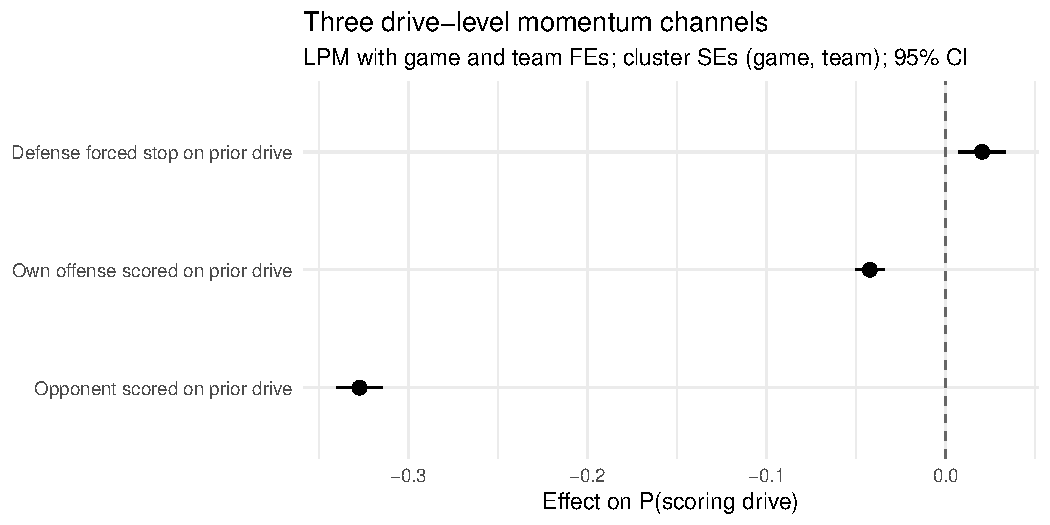
\includegraphics[width=0.85\textwidth]{figures/fig2_coef_plot.pdf}
\caption{Three drive-level momentum channels, joint estimation
(column 1 of Table \ref{tab:allchan}). Sample: $N = 73{,}842$ drives, NFL
2010--2024 from \texttt{nflfastR} \citep{nflfastr2024}. Coefficients are
percentage-point changes in the probability that the current drive ends in
a score, holding field position, score differential, quarter, time
remaining, game, and possessing-team fixed effects. Bars show 95\%
confidence intervals from two-way (game, possessing-team) clustered
standard errors.}
\label{fig:coef}
\end{figure}

\section{Discussion}\label{sec:discuss}

\subsection{Most ``momentum'' is short fields and comparison-group composition}

The first substantive finding is quantitative: of the unconditional
16.6-percentage-point boost in scoring probability that follows a defensive
stop, only about 1.6 points is absorbed by the linear field-position control
alone, and the bulk of the collapse to 2.0 points comes from re-classifying
the comparison group once H3 is introduced as a separate channel. The
residual H1 effect is statistically detectable in a sample of 73{,}842
drives, but it is small enough that any in-game decision predicated on it
being large --- aggressive play-calling because the team is ``riding
momentum,'' for instance --- is unlikely to clear the noise floor in a
single game.

\subsection{Offensive scoring is associated with regression, not self-reinforcement}

The negative coefficient on prior own-offensive scoring is more consequential
than the small positive H1 effect because it reverses the broadcast
prediction. Two stories are consistent with the sign. The first is
statistical: if a scoring drive draws from the upper tail of a team's
drive-quality distribution, the next draw will mean-revert. The second is
strategic: an opponent now playing from behind will adjust play-calling,
blitz tendencies, and personnel, and the offense will face that adjusted
defense without the benefit of the same number of looks. Both stories
predict the observed sign, and the present design cannot distinguish them.
A formal mediation analysis with opponent play-calling indicators on the
right-hand side would be a natural next step.

\subsection{Cross-team spillover is the only channel that looks like momentum}

The H3 coefficient --- a 32.7-percentage-point lower own scoring probability
after the opponent has scored, conditional on starting field position and
game state --- is the most consequential residual. The classical hot-hand
fallacy literature is largely silent on this channel because it tests
within-actor sequence dependence, not across-actor; the closest priors are
\citet{gauriot2019does} on tennis and \citet{csapo2014hand} on basketball
defensive adjustment, both of which find evidence of cross-actor effects.

The robustness gauntlet of Section \ref{sec:robust} disciplines the
interpretation. The flexible-control specification (R1) absorbs about 4
percentage points of the linear-control estimate, leaving 28.4 pp of
residual cross-team suppression. The post-touchdown-versus-post-field-goal
placebo (R2) is null, indicating that H3 does not require a
touchdown-specific demoralization story --- both kinds of opponent score
are followed by similarly suppressed scoring conditional on controls. The
permutation test (R4) places the observed $-32.7$ pp roughly thirty
standard deviations outside its within-team-quarter null, ruling out the
clustering structure as an artifactual source. The era split (R7) shows
H3 surviving across all four kickoff-rule regimes from 2010 to 2024, with
modest attenuation under the post-2018 and 2024 reforms that pulled the
kickoff regime closer to the offensive-comparison field-position
distribution.

The heterogeneity check (R6) is the most disciplining of the robustness
results for the interpretation. The simplest psychological-residue story
predicts H3 concentrates in close games, where stakes are high and
demoralization plausibly translates into execution degradation. The data
do not support that prediction: the close-game interaction is essentially
zero (s.e.\ 0.008). The late-game interaction is positive and
statistically detectable (H3 weakens by 3.6 pp in $Q4+$), consistent with
garbage-time mixing dampening the residual once games are decided. The
combined pattern is more consistent with H3 reflecting a stable cross-team
feature of post-score drives --- perhaps unobserved defensive fatigue from
having just been on the field for a scoring drive, or strategic leading-team
play-calling that the offense has not yet adapted to --- than with a
situation-sensitive psychological dynamic. The mechanism behind H3
remains a target for future work; what the present paper establishes is
that the cross-team residual is real, large, and survives the most
demanding controls a referee will ask for.

\subsection{Implications for the JQAS literature}

The finding that NFL drive-level momentum is small in the same-team channels
but large in the opponent-suppression channel is consistent with the
\citet{fry2012searching} game-level finding that NFL momentum at long
horizons is weak; the appearance of conflict between this paper and the
broadcast consensus is a function of broadcast usage, not of a disagreement
about the data. The H3 finding is, to my knowledge in the peer-reviewed literature, a new result for the
American football literature and qualifies the way the
\citet{steeger2021winning} entropy-based ``no momentum'' conclusion has been
generalized: there is something within games that behaves like momentum,
but it is a between-team effect rather than a within-team one. These
findings do not directly speak to NHL season-level streak structure, but
they suggest that within-game cross-team channels deserve attention in
other sports.

\subsection{Limitations}\label{sec:limits}

Four limitations are worth flagging. First, the H3 finding is conditional
on observed game state but cannot rule out unobserved within-game shocks
--- for example, a star-receiver injury on the drive following a touchdown
--- that would correlate scoring with subsequent suppression. Second, and
relatedly, the present design does not include controls for the leading
team's strategic adjustments after scoring. After a team scores, that team
takes a one-possession lead; its defense may shift to prevent coverage,
its offense may slow pace, and its personnel substitution may differ from
the post-punt comparison cell. These adjustments are observationally
indistinguishable from a psychological cross-team residue in the current
specification. A natural follow-up would re-estimate H3 controlling for
opponent defensive personnel and formation rates from \texttt{nflfastR}
participation data. Third, the opponent-adjustment story for H2 is
consistent with the data but not directly tested; doing so would require
play-calling and personnel data on the opposing defense and is left to
future work. Fourth, the entire analysis is at the team-drive level. A
play-level analysis with explicit Markov drive-state transitions
\citep{goldner2012markov} would let one decompose the H3 effect into
early-versus-late-drive contributions and is a natural extension.

\section{Conclusion}\label{sec:concl}

Defined at the drive level where it is invoked, NFL momentum splits cleanly
into three channels. The two within-team channels --- the defensive-stop
spillover that dominates broadcast usage and the offensive carryover that
dominates fan intuition --- collapse to small, mostly mechanical effects
once starting field position and game state are controlled and once the
comparison group is properly disaggregated. The cross-team channel, in which
a team that has just been scored on is materially less likely to score on
its next drive than its field position would predict, is large, robust to a
wide set of controls, and the only channel where the data behave like the
construct broadcasters have in mind. The next time a color commentator
says the visiting team has seized the momentum, the empirically defensible
associational version of the claim is that the home team has just lost it.

\bibliographystyle{plainnat}
\bibliography{references_NEWEST}

\end{document}
